\documentclass[a4paper, 12pt]{article}

\usepackage[portuges]{babel}
\usepackage[utf8]{inputenc}
\usepackage{amsmath}
\usepackage{indentfirst}
\usepackage{graphicx}
\usepackage{multicol,lipsum}
\usepackage[hidelinks]{hyperref}
\usepackage{circuitikz}
\usepackage{xcolor}
\usepackage{mdframed}
\usepackage{framed}

\begin{document}
%\maketitle

\begin{titlepage}
	\begin{center}
	
	%\begin{figure}[!ht]
	%\centering
	%\includegraphics[width=2cm]{c:/ufba.jpg}
	%\end{figure}

		\Huge{Universidade Federal do Espírito Santo}\\
		\large{Relatório do Trabalho de Eletricidade Aplicada}\\ 
		\vspace{15pt}
        \vspace{95pt}
        \textbf{\LARGE{Transformadores}}\\
		%\title{{\large{Título}}}
		\vspace{3,5cm}
	\end{center}
	
	\begin{flushleft}
		\begin{tabbing}
			Alunos: André Neves Prestes, Tiago da Cruz Santos e Victor David Lima\\
			Professor : Rosane Bodart Soares\\
	\end{tabbing}
 \end{flushleft}
	\vspace{1cm}
	
	\begin{center}
		\vspace{\fill}
			 Junho\\
		 2019
			\end{center}
\end{titlepage}
%%%%%%%%%%%%%%%%%%%%%%%%%%%%%%%%%%%%%%%%%%%%%%%%%%%%%%%%%%%

% % % % % % % % %FOLHA DE ROSTO % % % % % % % % % %

\begin{titlepage}
	\begin{center}
	
	%\begin{figure}[!ht]
	%\centering
	%\includegraphics[width=2cm]{c:/ufba.jpg}
	%\end{figure}

	\Huge{Universidade Federal do Espírito Santo}\\
		\large{Relatório do Trabalho de Eletricidade Aplicada}\\  
\vspace{15pt}
        
        \vspace{85pt}
        
		\textbf{\LARGE{Relatório}}
		\title{\large{Título}}
	%	\large{Modelo\\
     %   		Validação do modelo clássico}
			
	\end{center}
\vspace{1,5cm}
	
	\begin{flushright}

   \begin{list}{}{
      \setlength{\leftmargin}{4.5cm}
      \setlength{\rightmargin}{0cm}
      \setlength{\labelwidth}{0pt}
      \setlength{\labelsep}{\leftmargin}}

      \item Relatório do Trabalho de Pesquisa sobre Transformadores Apresentado pelos alunos de Ciências da Computação da Universidade Federal Do Espírito Santo.

      \begin{list}{}{
      \setlength{\leftmargin}{0cm}
      \setlength{\rightmargin}{0cm}
      \setlength{\labelwidth}{0pt}
      \setlength{\labelsep}{\leftmargin}}

			\item Alunos: André Neves Prestes, Tiago da Cruz Santos e Victor David Lima\
            \item Professor : Rosane Bodart Soares\

      \end{list}
   \end{list}
\end{flushright}
\vspace{1cm}
\begin{center}
		\vspace{\fill}
		 Junho\\
		 2019
			\end{center}
\end{titlepage}
\newpage
% % % % % % % % % % % % % % % % % % % % % % % % % %
\newpage
\tableofcontents
\thispagestyle{empty}

\newpage
\pagenumbering{arabic}
% % % % % % % % % % % % % % % % % % % % % % % % % % %
\section{Introdução}

\paragraph{}Neste relaório falaremos sobre Transfomadores e diversos assuntos relacionados a eles.

\paragraph{}A estrutura fisíca de um Transformador é basicamente formada por um ferro enrolado por fios, de modo que esses fios são divididos em dois enrolamentos, o primário(com um número Np de espiras) ligado a fonte de tensão e o secundário(com um número Ns de espiras) ligada a carga, sendo a relação entre as suas tensões e correntes definida de acordo com o número de espiras presentes em cada um deles e tensão que o enrolamento primário esta ligado. Desta forma:\\

\begin{mdframed}[backgroundcolor=gray!20]
\begin{center}
		$V_s$ = $V_p$ $\dfrac{N_s}{N_p}$ (transformação da tensão)
			\end{center}
    \begin{center}
		$I_s$ = $I_p$ $\dfrac{N_s}{N_p}$ (transformação da corrente)
			\end{center}
\end{mdframed}
	

\paragraph{}A base teórica para o funcionamento de um transformador é a de que este é um dispositivo magnético que tira proveito fenômeno da indutância mútua, em que este ocorre quando duas ou mais bobinas(fios enrolados ao núcleo) estão proximos umas das outras de modo que o fluxo magnetico atraves da bobina não depende somente da corrente nesta, mas também das correntes presentes nas outras bobinas correlacionadas. Desta forma o campo magnetico que passa pelas bobinas é a superposição de todos os campos magneticos das bobinas associadas. \\
\newpage
\section{Conceitos de Eletromagnetismo}
    \subsection{Campo Magnético}
\paragraph{}A respeito de campos magneticos em eletromagnetismo foi descoberto que um campo magnético $\overrightarrow{B}$ é gerado por cargas magnéticas (conhecidas como monopolos magnéticos), entretanto, embora a exitencia destas seja prevista em algumas teorias, essas cargas ate hoje não foram observadas. Deste modo os campos magneticos são criados de duas formas.

\paragraph{}A primeira forma consiste em usar partículas eletricamente carregadas em movimento, como os elétrons responsáveis pela corrente elétrica em um fio, para fabricar um eletroímã, sendo que o campo magnético é produzido pela corrente.

\paragraph{}A outra forma de produzir um campo magnético se baseia no fato de que muitas partículas elementares possuem um campo magnético próprio. O campo magnético é uma propriedade básica das partículas elementares, como a massa e a carga elétrica, em alguns materiais os campos magnéticos dos elétrons se somam para produzir um campo magnético no espaço que cerca o material. Sendo esse o motivo da existencia de imãs permanentes, com campos magneticos permanentes. Porém, em grande parte dos materiais, os campos magneticos dos eletrons se cancelam, assim tornando o campo magetico em torno do material nulo. 

\paragraph{}\textbf{Partícula Carregada em Movimento:} $\overrightarrow{B}$ é definido em principio, medindo a força $\overrightarrow{F_B}$ que age sobre a partícula quando ela passa, com várias velocidades e direções, pelo ponto no qual $\overrightarrow{B}$ esta sendo medido. Depois de realizados varios experimentos deste tipo, foi constatado que, qunado a velocidade $\overrightarrow{v}$ da partícula tem certa direção a força $\overrightarrow{F_B}$ é nula. Porém para o resto das direções de $\overrightarrow{v}$, o modulo de $\overrightarrow{F_B}$ é proporcional a v$\cdot$ sen($\phi$), sendo $\phi$ o ângulo entre a direção em que a força é zero e a direção de $\overrightarrow{v}$. Além disso, a direção de $\overrightarrow{F_B}$ é sempre perpendicular à direção de $\overrightarrow{v}$, assim sugerindo que produto vetorial esta envolvido.

\paragraph{}\textbf{O Campo:} É possivel definir um campo magnetico $\overrightarrow{B}$ como uma grandeza vetorial em que a direção coincide com aquela para a qual a força é zero. Deste modo o módulo de $\overrightarrow{B}$ em termos do módulo da força:
\\
\begin{mdframed}[backgroundcolor=gray!20]
\begin{center}
	B = $\dfrac{F_B}{|q|\cdot v}$
			\end{center}
\end{mdframed}

\paragraph{}Em que q é a carga da particula.

\paragraph{}Podemos expressar esses resultados usando a seguinte equação vetorial: \\
\begin{mdframed}[backgroundcolor=gray!20]
\begin{center}
	$\overrightarrow{F_B} = q\overrightarrow{v} \cdot \overrightarrow{B}$
    \\e\\
    $F_B = |q| \cdot v \cdot B \cdot sen(\phi)$
			\end{center}
\end{mdframed}

\paragraph{}Onde $\phi$ é o ângulo entre as direções da velocidade e do campo magnético $\overrightarrow{B}$.

\subsection{Lei de Ampère}

\paragraph{} Em eletromagnetismo é possivel obter o campo magnético total relacionado a qualquer distribuição de correntes somando os campos magnetico elementares d$\overrightarrow{B}$ gerados por todos os elementos de corrente i d$\overrightarrow{s}$. No caso de distribuições mais complexas é necessario a utilização de um computador. Contudo, na ocorrência de certos tipos de simetria, podemos usar a \textbf{Lei de Ampère} para calcular diretamente o campo magnetico total. De modo que a lei é expressa por:
\begin{mdframed}[backgroundcolor=gray!20]
\begin{center}
		\quad $\oint{\overrightarrow{B}}\cdot d\overrightarrow{s}= \oint{B}\cdot cos(\theta) \cdot ds =\mu _{0}I$  (Lei de Ampère)
		\end{center}
\end{mdframed}
    
   	
\paragraph{}O círculo no sinal de integral indica que a integração do produto escalar $\overrightarrow{B}\cdot d\overrightarrow{s}$ deve ser realizada para uma curva fechada, conhecida como amperiana. A corrente i no lado direito da equação é a corrente total envolvida pela amperiana, o $\mu _{0}$ sendo a permeabilidade magnética no vácuo com um valor no Sistema Internacional de Unidades (SI):
\\
\begin{mdframed}[backgroundcolor=gray!20]
\begin{center}
    ${\displaystyle \mu _{0}=4\pi \times 10^{-7}{\frac {\text{N}}{{\text{A}}^{2}}}}$.
    \end{center}
\end{mdframed}
 
	\paragraph{}E $\theta$ referindo-se ao angulo entre $\overrightarrow{B}$ e d$\overrightarrow{s}$.
   
\paragraph{}Para entender melhor o significado do produto escalar $\overrightarrow{B}\cdot d\overrightarrow{s}$ e sua integral, vamos aplicar a Lei de Ampère à situação da figura abaixo, conforme o exemplo presente no livro Fundamentos de Circuitos Elétricos no capitulo 29-3. \\

\begin{figure}[h]
    \begin{center}
        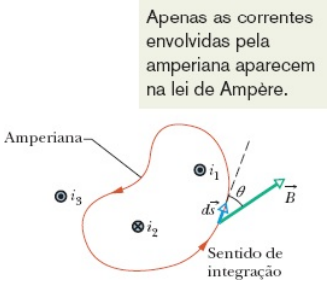
\includegraphics[width=60mm]{Capturar.PNG}
    \end{center}
    \caption{Exemplo Geral}
    \label{Fig. Exemplo}
\end{figure}

\paragraph{} A figura mostra a seção reta de três fios longos, perpendiculares ao plano do papel, percorridos por correntes i1, i2 e i3. Uma amperiana arbitrária traçada no plano do papel envolve duas das correntes, mas não a terceira. O sentido anti-horário indicado na amperiana mostra o sentido arbitrariamente escolhido para realizar a integração da equação da Lei de Ampère. Para aplicarmos tal lei é necessario dividir a amperiana em elementos de comprimento $d\overrightarrow{s}$, que são tangentes a curva e apontam no sentido de integração.

\paragraph{} Suponha que, no local do elemento $d\overrightarrow{s}$ que aparece na figura, o campo magnetico total gerado devido as correntes nos três fios seja $\overrightarrow{B}$. Como os fios são perpendiculares ao plano do papel, sabemos que os campos magnéticos em $d\overrightarrow{s}$ produzidos pelas três correntes estão no plano da figura, assim, o campo magnético total também deve estar nesse plano, porém não conhecendo a orientação de $\overrightarrow{B}$, desta forma sendo desenhado arbitrariamente na Figura 1.

\paragraph{} \textbf{Sinal das Correntes:} Para executar a integração, não precisamos conhecer o sentido de $\overrightarrow{B}$ em todos os pontos da amperiana; supomos arbitrariamente que o sentido de $\overrightarrow{B}$ coincide com o sentido de integração, como na Figura 1, e usamos a seguinte regra da mão direita para atribuir um sinal positivo ou negativo às correntes que contribuem para a corrente total envolvida pela amperiana, i:\\

\begin{mdframed}[backgroundcolor=gray!20] 
         Apoie a palma da mão direita na amperiana, com os dedos apontando no sentido da integração. Uma corrente no sentido do polegar estendido recebe sinal positivo; uma corrente no sentido oposto recebe sinal negativo.
    \end{mdframed}
    
\paragraph{}Com isso resolvemos a equação da Lei de Ampère para obter o módulo de $\overrightarrow{B}$. Se B é positivo, isso significa que o sentido escolhido para $\overrightarrow{B}$ está correto; se B é negativo, ignoramos o sinal e tomamos $\overrightarrow{B}$ com o sentido oposto.

\paragraph{}\textbf{Corrente Total:} Aplicando a regra da mão direita da Lei de Ampère na situação da Figura 1, tomando o sentido de integração como o sentido anti-horário, a corrente total envolvida pela amperiana é:

\begin{mdframed}[backgroundcolor=gray!20]
\begin{center}
    i = $i_1$ - $i_2$
    \end{center}
\end{mdframed}
	
\paragraph{}(A corrente i3 está do lado de fora da amperiana.) Deste modo:


	\begin{mdframed}[backgroundcolor=gray!20]
	\begin{center}
		\quad $\oint{\overrightarrow{B}}\cdot d\overrightarrow{s}=\mu _{0}\cdot$ ($i_1$ - $i_2$)  (Lei de Ampère)
		\end{center}
\end{mdframed}

\paragraph{}A corrente $i_3$ não é levada em consideração na equação acima pois suas contribuições para o campo magnético se cancelam quando a integração da equação acima é realizada para uma curva fechada, o que não ocorre para as correntes presentes no interior da amperiana.



    \subsection{Lei de Faraday}

\paragraph{}Faraday descobriu que uma força eletromotriz e uma corrente podem ser induzidas em uma espira, quando se varia a quantidade de campo magnético que atravessa a espira. Faraday percebeu ainda que a “quantidade de campo magnético” pode ser visualizada em termos das linhas de campo magnético que atravessam a espira. A lei de indução de Faraday, quando aplicada a
nossos experimentos, diz o seguinte:
\\
\begin{mdframed}[backgroundcolor=gray!20]
	\begin{center}
		Uma força eletromotriz é induzida na espira quando varia-se o número de linhas de campo magnético que atravessam a mesma.
		\end{center}
\end{mdframed}

\paragraph{}O número de linhas de campo que atravessam a espira não importa, de modo que os valores da força eletromotriz e da corrente induzida são determinados pela taxa de variação desse número.

\paragraph{}Assim, quando um polo norte de um imã se aproxima da espira o número de linha de campos que atravessam a espira aumentão. Esse aumento faz com que os elétrons de condução se movam (ou seja, produz uma corrente induzida) e fornece a energia necessária para esse movimento (ou seja, produz uma força eletromotriz induzida). Quando o ímã para de se mover, o número de linhas de campo que atravessam a espira deixa de variar e a corrente induzida e a força eletromotriz induzida desaparecem.

\paragraph{}Deste modo, usando a definição de fluxo magnetico:  
\\
\begin{mdframed}[backgroundcolor=gray!20]
	\begin{center}
		$\phi_B = \int \overrightarrow{B} \cdot d\overrightarrow{A} $ (fluxo magnetico através da área A)
		\end{center}
\end{mdframed}

\paragraph{}em que d$\overrightarrow{A}$ é um vetor de módulo dA perpendicular a um elemento de área dA.

\paragraph{}Podemos enunciar a Lei de Faraday como:
\\
\begin{mdframed}[backgroundcolor=gray!20]
	\begin{center}
		O módulo da força eletromotriz induzida em uma espira condutora é igual à taxa de variação, com o tempo,do fluxo magnético $\phi_B$ que atravessa a espira.
		\end{center}
\end{mdframed}

\paragraph{}Como a força eletromotriz induzida $\mathcal  {E}$ se opõe a variação do fluxo, a Lei de Faraday é representada matematicamente por:
\\
\begin{mdframed}[backgroundcolor=gray!20]
	\begin{center}
		$\mathcal  {E}$ = - $\dfrac{d \phi_B}{dt}$ (Lei de Faraday)
		\end{center}
\end{mdframed}

\paragraph{}Se ocorrer um a variação de fluxo magnetico em uma bobina de N espiras, uma força eletromotriz é induzida em cada espira e a força eletromotriz total é a soma dessas forças eletromotrizes. Se as espiras da bobina estão muito próximas (ou seja, se temos um enrolamento compacto), o mesmo fluxo magnético $\phi_B$ atravessa todas as espiras, e a força eletromotriz total induzida na bobina é dada por:
\\
\begin{mdframed}[backgroundcolor=gray!20]
	\begin{center}
		$\mathcal  {E}$ = - N $\dfrac{d \phi_B}{dt}$
		\end{center}
\end{mdframed}

\paragraph{}Deste modo, é possivel alterar o fluxo magnetico de três formas:
\begin{enumerate}
    \item Mudar o módulo B do campo magnético.
    \item Mudar a área total da bobina ou a parte da área atravessada pelo campo magnético (aumentando ou diminuindo o tamanho da bobina no primeiro caso e colocando uma parte maior ou menor da bobina na região onde existe o campo no segundo).

    \item Mudar o ângulo entre a direção do campo magnético e o plano da bobina (fazendo girar a bobina, por exemplo).

\end{enumerate}

    \subsection{Lei de Lenz}
\paragraph{}A partir da Lei de Faraday, foi criada a Lei de Lenz para determinar o sentido da corrente induzida na espira:
\\
\begin{mdframed}[backgroundcolor=gray!20]
	\begin{center}
		A corrente induzida em uma espira tem um sentido tal que o campo magnético produzido pela corrente se opõeao campo magnético que induz a corrente.
		\end{center}
\end{mdframed}

\paragraph{}Apesar da força eletromotriz induzida tem um sentido compatível com o sentido da corrente induzida, a ideia por traz da Lei de Lenz é a de oposição. Para melhor entendimento de tal funcionamento iremos usar o exemplo no qual um imã se aproxima de uma espira condutora:
\begin{enumerate}
    \item \textbf{Oposição ao Movimento de um Polo:} Como visto na Lei de Faraday a aproximação ou afastamento de um imã de uma espira gera uma variação no fluxo magnetico que atravessa a espira, assim induzindo uma corrente. Apos ser percorrida por tal corrente a espira começa a se comportar como um dipolo magnético com um polo sul e um norte. Deste modo apresentando momento magnético $\overrightarrow{\mu}$, que pode ter o sentido do polo norte para o sul ou ao contrario, dependendo se o imã esta se aproximando ou se afastando, com o polo norte ou polo sul. Com o intuito de se opor ao aumento de fluxo causado pelo imã, o polo da espira deve estar voltada ao polo do imã, sendo os dois polos de mesma polaridade em caso da aproximação do imã, ou opostos no caso de afastamento do mesmo.
    \item \textbf{Oposição à Variação de Fluxo:} Com o ímã inicialmente distante, o fluxo magnético que atravessa a espira é zero. Quando o polo norte do ímã se aproxima da espira com o campo magnético $\overrightarrow{B}$ apontando para baixo, o fluxo através da espira aumenta. Para se opor a esse aumento de fluxo, a corrente induzida i deve criar um campo $\overrightarrow{B_ind}$ apontando para cima, nesse caso, o fluxo para cima de $\overrightarrow{B_ind}$ se opõe ao aumento do fluxo para baixo causado pela aproximação do ímã e o consequente aumento de $\overrightarrow{B}$.
\end{enumerate}

\paragraph{}\textbf{Atenção:} O fluxo de $\overrightarrow{B_ind}$ sempre se opõe à variação do fluxo de $\overrightarrow{B}$, mas isso não significa que $\overrightarrow{B}$ e $\overrightarrow{B_ind}$ sempre têm sentidos opostos. 
\\
\begin{figure}[h]
    \begin{center}
        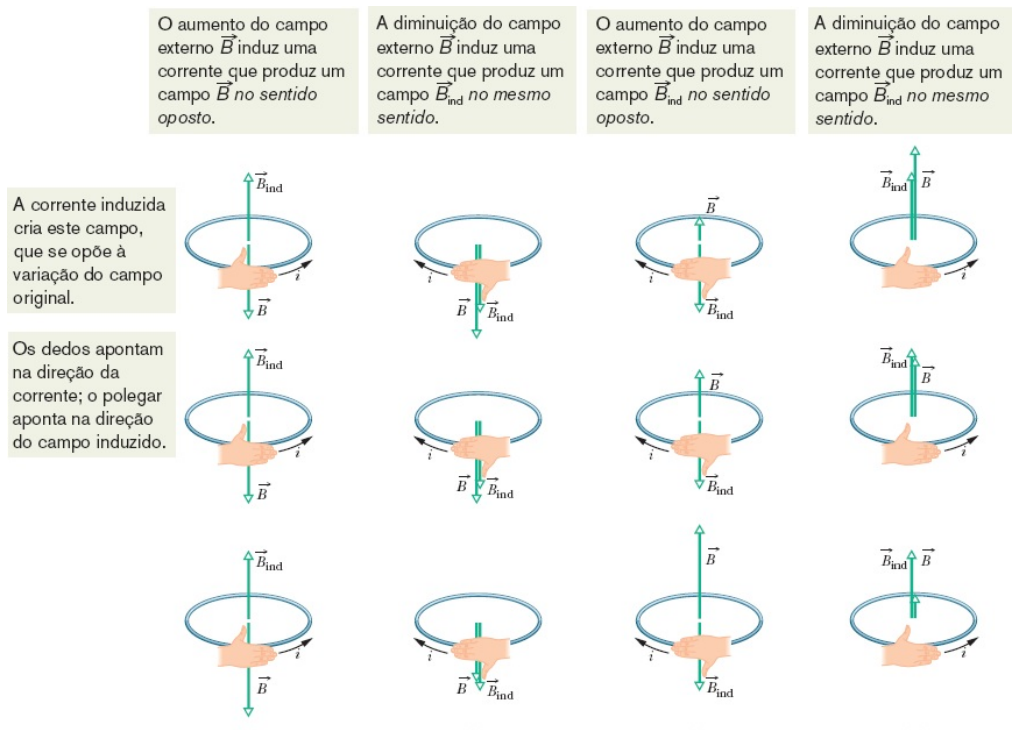
\includegraphics[width=170mm]{novo.PNG}
    \end{center}
    \caption{Regra da mão direita}
    \label{Fig. Exemplo}
\end{figure}

    \newpage
    \subsection{Principio de Funcionamento do Transformador}
    \paragraph{}Tranfomadores são circuitos que afetam um ao outro usando o conceito de campo magnético. O principio de funcionamento de um transformador é baseado nas leis de Faraday e Lenz, as leis do eletromagnetismo e da indução eletromagnética.
\paragraph{}Tranformadores simples possuem 2 enrolamentos ou bobinas enrodaos em um único núcleo, sendo chamados de enrolaento primario e secundario. Quando uma corrente CA é aplicada no enrolamento primario, o campo magnético criado pelo primario causa o surgimento de uma tensão no secundario, fenomeno conhecido como \textit{Indutancia mutua}.
\paragraph{}Transformadores são utilizados por sistemas de gearação de energia para diminuir tensões que serão entregues aos clientes, por receptores de rádio e TV para casamento de impedãncias, que serão vistas na seção \ref{impedCas}.%tem mais coisa ainda calma
\subsubsection{Indutância mutua}
\begin{center}
\begin{circuitikz}[american voltages]
\draw
(0,-3) to [american current source, l=$i(t)$] (0, 0)
(0, 0) to [short, -] (3, 0)
to [short, -] (3, 0)
to [L, -, v_>=$V_1$, l=$N_1$, f=$I_1$] (3, -3)
(0, -3) to [short, -] (3, -3)
to [short, -] (3, -3)
(5, 0) to [L, -, v^>=$V_2$, l_=$N_2$] (5, -3)
(5, 0) to [short, -*] (6, 0)
(5, -3) to [short, -*] (6, -3);
\end{circuitikz}
\end{center}
\paragraph{}Quando 2 indutores são colocados lado a lado, uma variação na corrente em um induzirá uma força eletromotriz no outro. O primeiro indutor possui uma corrente $I_1$ e possui $N_1$ voltas que gera um campo magnético. Já que os induores estão próximos, algumas linhas do campo magnético do primeiro irão passar pelo segundo. Como a corrente $I_1$ varia com o tempo, o campo gerado pelo indutor primario também irá variar, gerando uma força eletromotriz no indutor secundário.\\
\begin{mdframed}[backgroundcolor=gray!20]
	\begin{center}
	\textbf{Indutância mútua} é a capacidade de um indutor induzir tensão em um indutor vizinho e essa grandeza é medida em henrys (H).
	\end{center}
\end{mdframed}
\paragraph{}Sendo $\phi_{21}$ o fluxo do campo magnético atravez do indutor secundario ocasionado pelo $I_1$ e fazedo $I_1$ variar no tempo, uma força eletromotriz induzida no induor secundario irá surgir.
\begin{mdframed}[backgroundcolor=gray!20]
	\begin{equation*}
    \varepsilon_{21} = -N_2\frac{d\phi_{21}}{dt}
    \end{equation*}
\end{mdframed}
\section{Isolação Térmica}
\newpage
\section{Transformador Ideal}
    \subsection{Equações Fundamentais}
    \subsection{Balanceamento de Potência}
    \subsection{Potência Complexa e Potência Aparente}
    \subsection{Conexão de Impedâncias no Secundário}
    \subsection{Casamento de Impedâncias Via Transformador} \label{impedCas}
\newpage
\section{Exemplos de Utilização}
\newpage
\section{Resolução de Exercícios}
\newpage

\section*{Bibliografia}
\addcontentsline{toc}{section}{Bibliografia}
\footnotesize{

\noindent 
K. ALEXANDER, Charles; N. O. SADIKU, Matthew.\textit{Fundamentos de Circuitos Elétricos}. 5º ed. Porto Alegre : AMGH, 2013.\\
\\
NILSSON, James W.; A. RIEDEL, Susan. \textit{Circuitos Elétricos}. 8º ed. São Paulo: Pearson Prentice Hall, 2009\\
\\
HALLIDAY, David; RESNICK, Robert; WALKER, Jearl. \textit{Fundamentos de Fisíca, volume 3}: Eletromagnetismo. 10º ed. Rio de Janeiro: LTC, 2016\\ 
\\
MARTIGNONI, Alfonso. \textit{Transformadores}. 8ª ed. São Paulo, Globo. 1991
}
\addcontentsline{toc}{section}{Anexo}
\end{document}



